\documentclass[11  pt]{article} 
\usepackage[lmargin=1in,rmargin=1.75in,bmargin=1in,tmargin=1in]{geometry}  


% For hyperlinking everything
\usepackage{hyperref}
\hypersetup{
	colorlinks=true, %set true if you want colored links
	linktoc=all,     %set to all if you want both sections and subsections linked
	linkcolor=blue,  %choose some color if you want links to stand out
}


\usepackage[latin1]{inputenc}
\usepackage{amsmath}
\usepackage{mathrsfs}  
\usepackage{amsfonts}
\usepackage{amssymb}
\usepackage{graphicx}
\usepackage{subfig}
\usepackage{caption}
\usepackage{algorithm}
%\usepackage{algcompatible}
%\usepackage{algorithmicx}
\usepackage{algpseudocode}

\usepackage{titlesec}
\titleformat{\section}{\fontfamily{lmss}\fontsize{14}{15}\bfseries}{\thesection}{1em}{}
\titleformat{\subsection}{\fontfamily{lmss}\fontsize{12}{15}\bfseries}{\thesubsection}{1em}{}




\usepackage{amsthm}

\newtheoremstyle{noit}
{10pt}% <Space above>
{10pt}% <Space below>
{}% <Body font>
{}% <Indent amount>
{\bfseries}% <Theorem head font>
{.}% <Punctuation after theorem head>
{.5em}% <Space after theorem headi>
{}% <Theorem head spec (can be left empty, meaning `normal')>

\newtheoremstyle{example}
{10pt}% <Space above>
{10pt}% <Space below>
{}% <Body font>
{20pt}% <Indent amount>
{\bfseries}% <Theorem head font>
{.}% <Punctuation after theorem head>
{.5em}% <Space after theorem headi>
{}% <Theorem head spec (can be left empty, meaning `normal')>


\newtheoremstyle{indented}{20pt}{20pt}{\addtolength{\leftskip}{2.5em}}{}{\bfseries}{.}{.5em}{}


\newtheorem{theorem}{Theorem}
\numberwithin{theorem}{section}
\newtheorem{lemma}[theorem]{Lemma}
\newtheorem{corollary}[theorem]{Corollary}
\newtheorem{observation}{Observation}
%\numberwithin{observation}{section}
%\numberwithin{definition}{section}
\newtheorem{conjecture}{Conjecture}
\newtheorem{Qu}{Question}
\newcommand{\QU}{\begin{Qu}\normalfont}

\theoremstyle{noit}
\newtheorem{fact}{Fact}
\newtheorem{definition}{Definition}

\theoremstyle{indented}
\newtheorem{example}{Example}

\theoremstyle{indented}
\newtheorem{problem}{Problem}


%\newenvironment{proof}{\noindent{\bf Proof:} \hspace*{1em}}{
%    \hspace*{\fill} $\Box$ }
%\newenvironment{proof_of}[1]{\noindent {\bf Proof of #1:}
%    \hspace*{1em} }{\hspace*{\fill} $\Box$ }
%\newenvironment{proof_claim}{\begin{quotation} \noindent}{
%    \hspace*{\fill} $\diamond$ \end{quotation}}
\newcommand{\vs}[1]{\vspace{#1}}

\newcommand{\lecture}[2]{
 \noindent
\begin{center}
	\framebox{
		\vbox{
			\hbox to 5.78in { {\bf CSCE 411: Design and Analysis of Algorithms} \hfill  }
			\vspace{2mm}
			\hbox to 5.78in { {\Large \hfill Lecture #1\hfill} }
			\vspace{2mm}
			\hbox to 5.78in { {\it Date: #2 \hfill Lecturer: Nate Veldt} }
		}
	}
\end{center}
\vspace*{4mm}
}


\newcommand{\hw}[2]{
	\noindent
	\begin{center}
		\framebox{
			\vbox{
				\hbox to 5.78in { {\bf CSCE 411: Design and Analysis of Algorithms} \hfill  }
				\vspace{2mm}
				\hbox to 5.78in { {\Large \hfill Homework #1\hfill} }
				\vspace{2mm}
				\hbox to 5.78in { {\it Due date: #2 \hfil} }
			}
		}
	\end{center}
	\vspace*{4mm}
}



\newcommand{\under}[1]{\underline{\hspace{#1}}}
\setlength{\parindent}{0em}

%\usepackage[tagged]{accessibility}

% Graph terms
\newcommand{\vol}{\textbf{vol}}
\newcommand{\cut}{\textbf{cut}}


% Matrices
\newcommand{\mA}{\textbf{A}}
\newcommand{\mB}{\textbf{B}}

% vectors
\newcommand{\ve}{\textbf{e}}
\newcommand{\vx}{\textbf{x}}


% Other
\newcommand{\calN}{\mathcal{N}}

\usepackage{mathtools}
\DeclarePairedDelimiter\ceil{\lceil}{\rceil}
\DeclarePairedDelimiter\floor{\lfloor}{\rfloor}


\newcommand*{\aitem}{ \item[{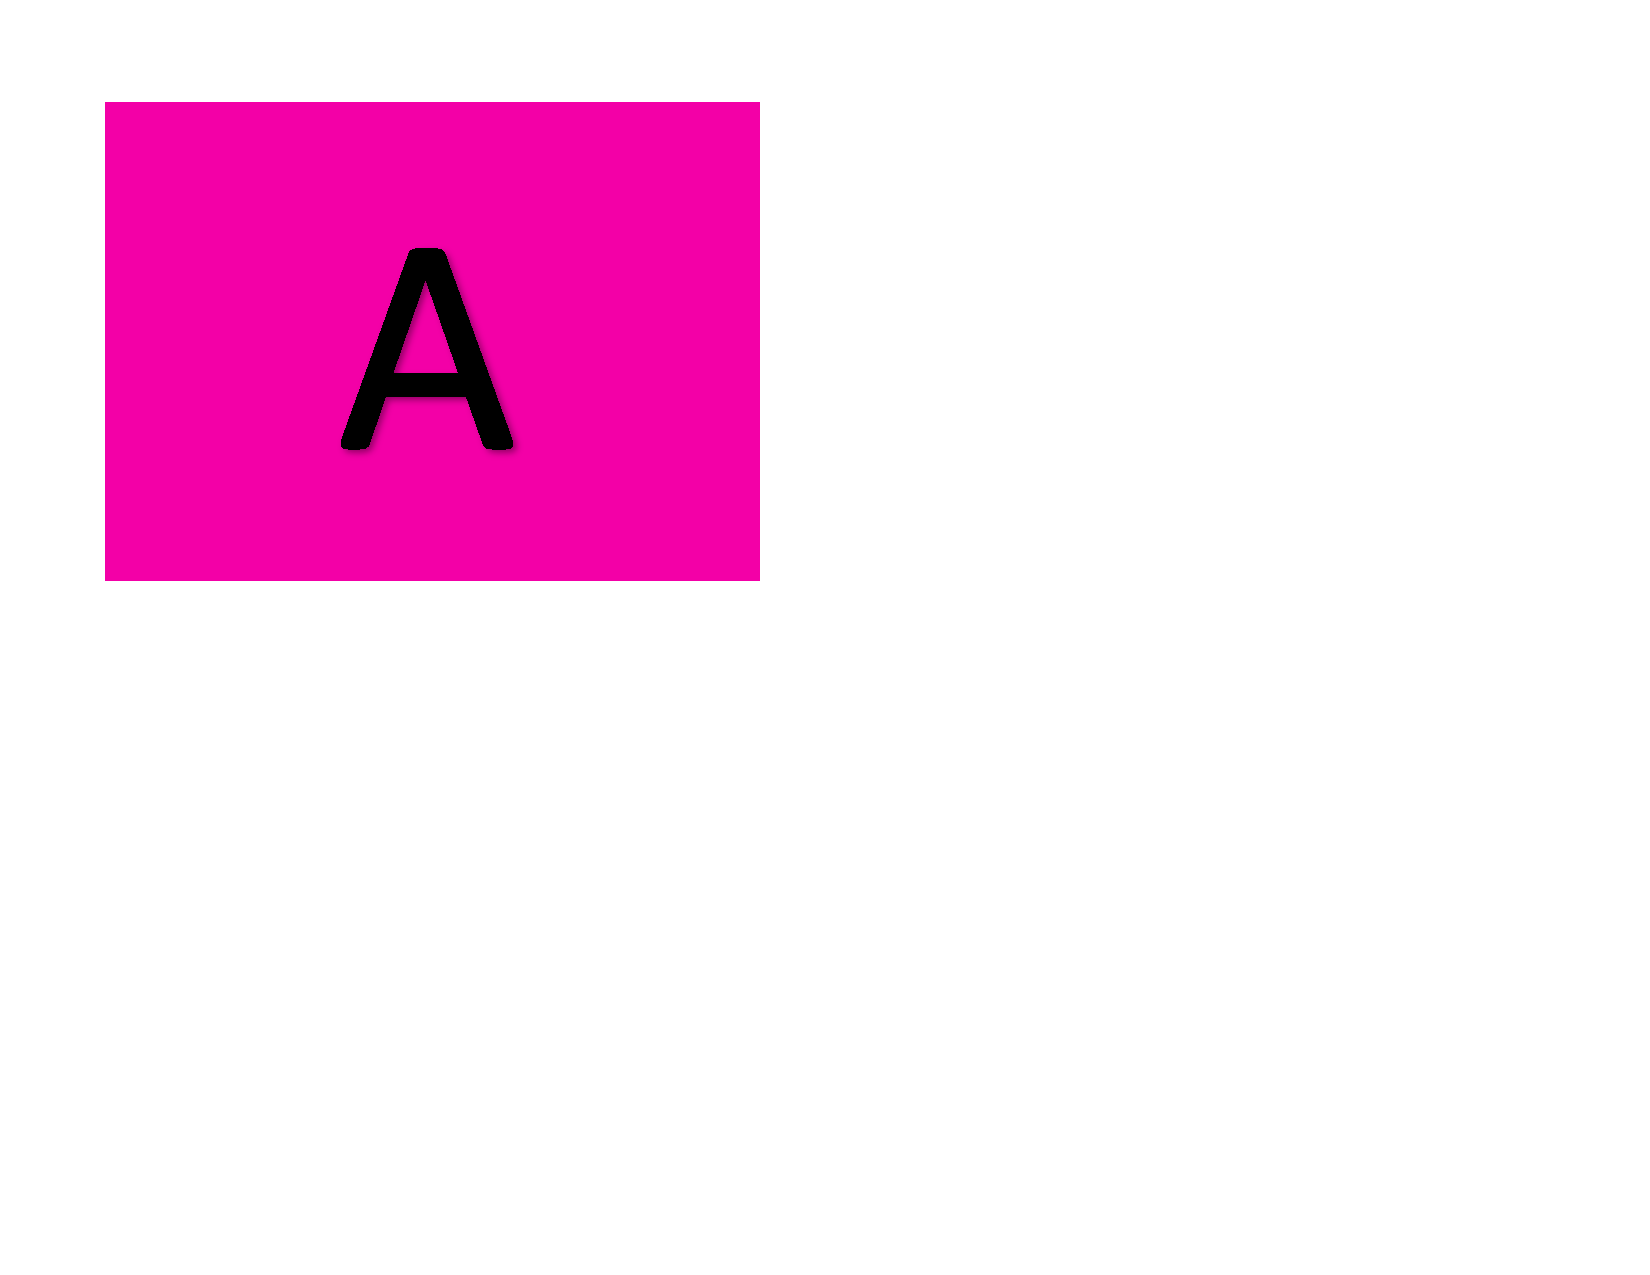
\includegraphics[width=0.8cm,height=0.5cm]{../../Lectures/figures/A}} ]  }
\newcommand*{\bitem}{ \item[{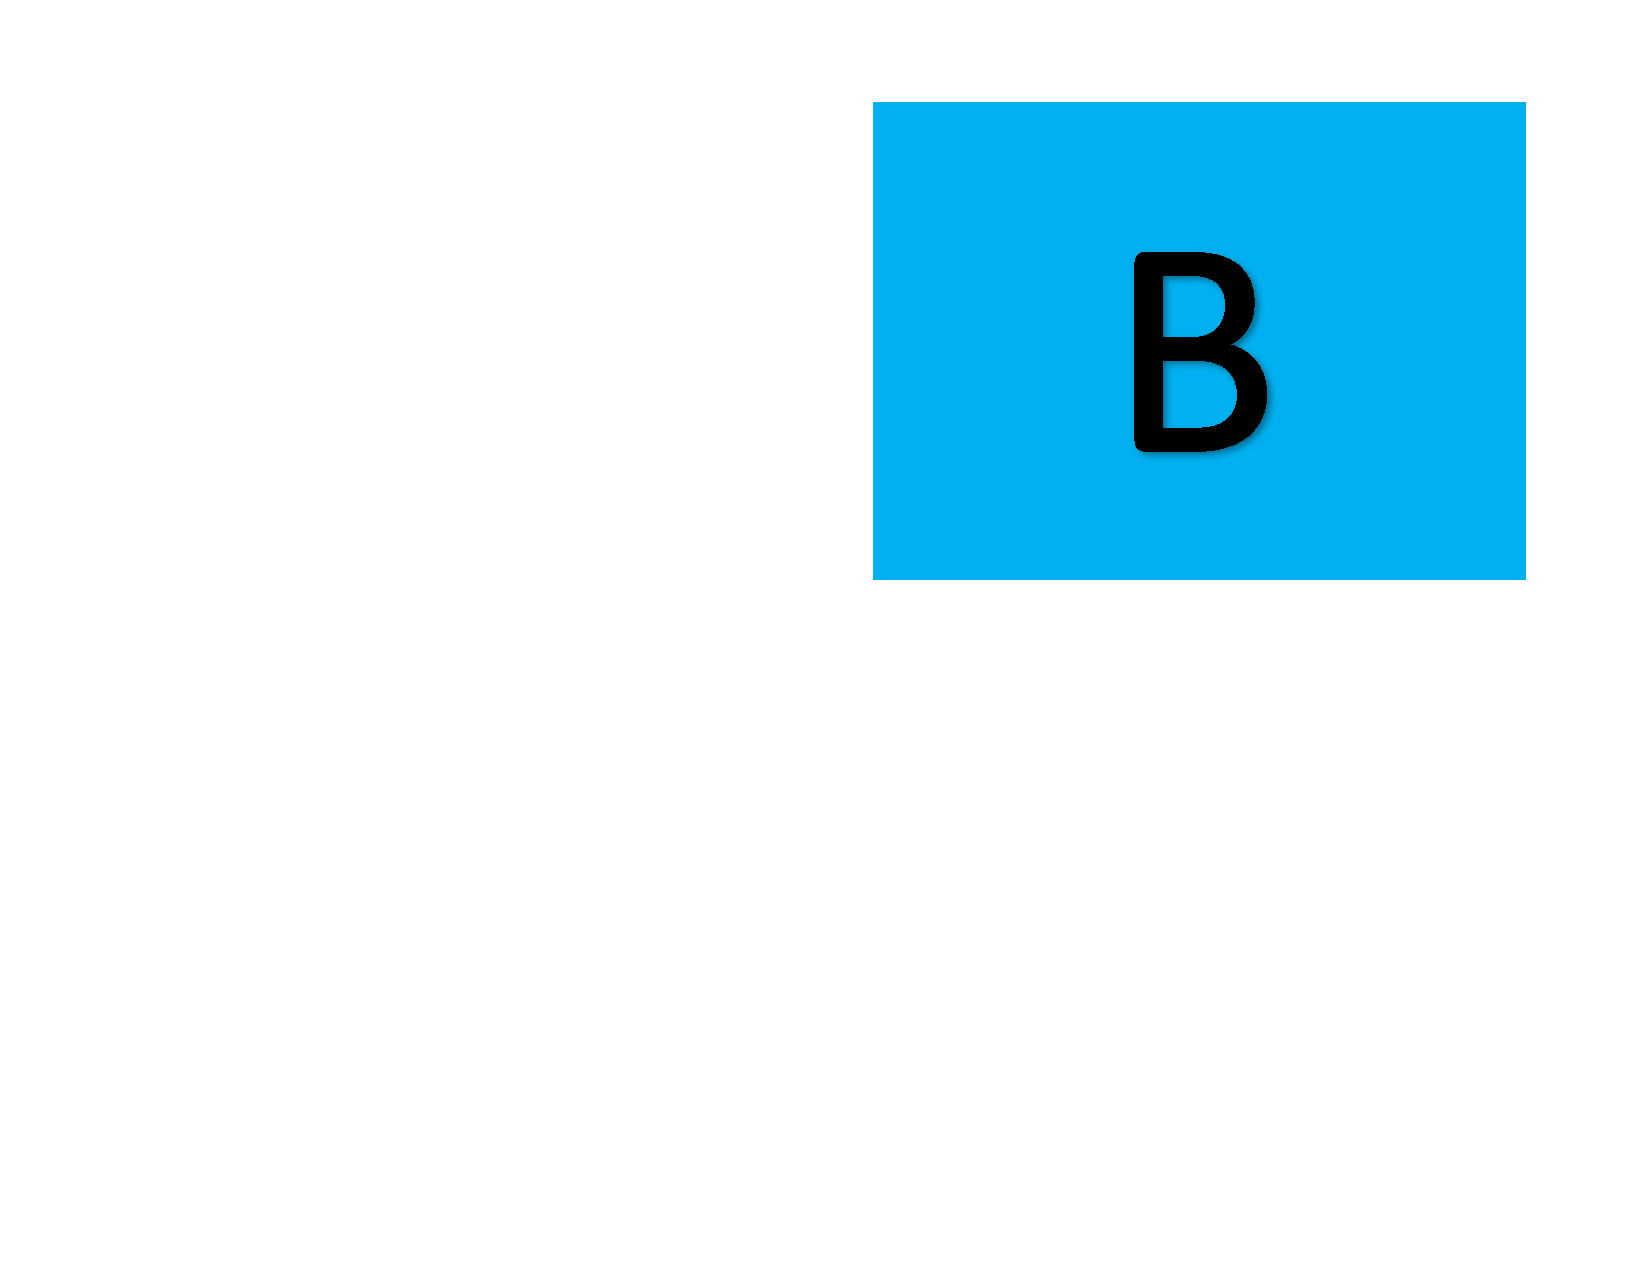
\includegraphics[width=0.8cm,height=0.5cm]{../../Lectures/figures/B}} ]  }
\newcommand*{\citem}{ \item[{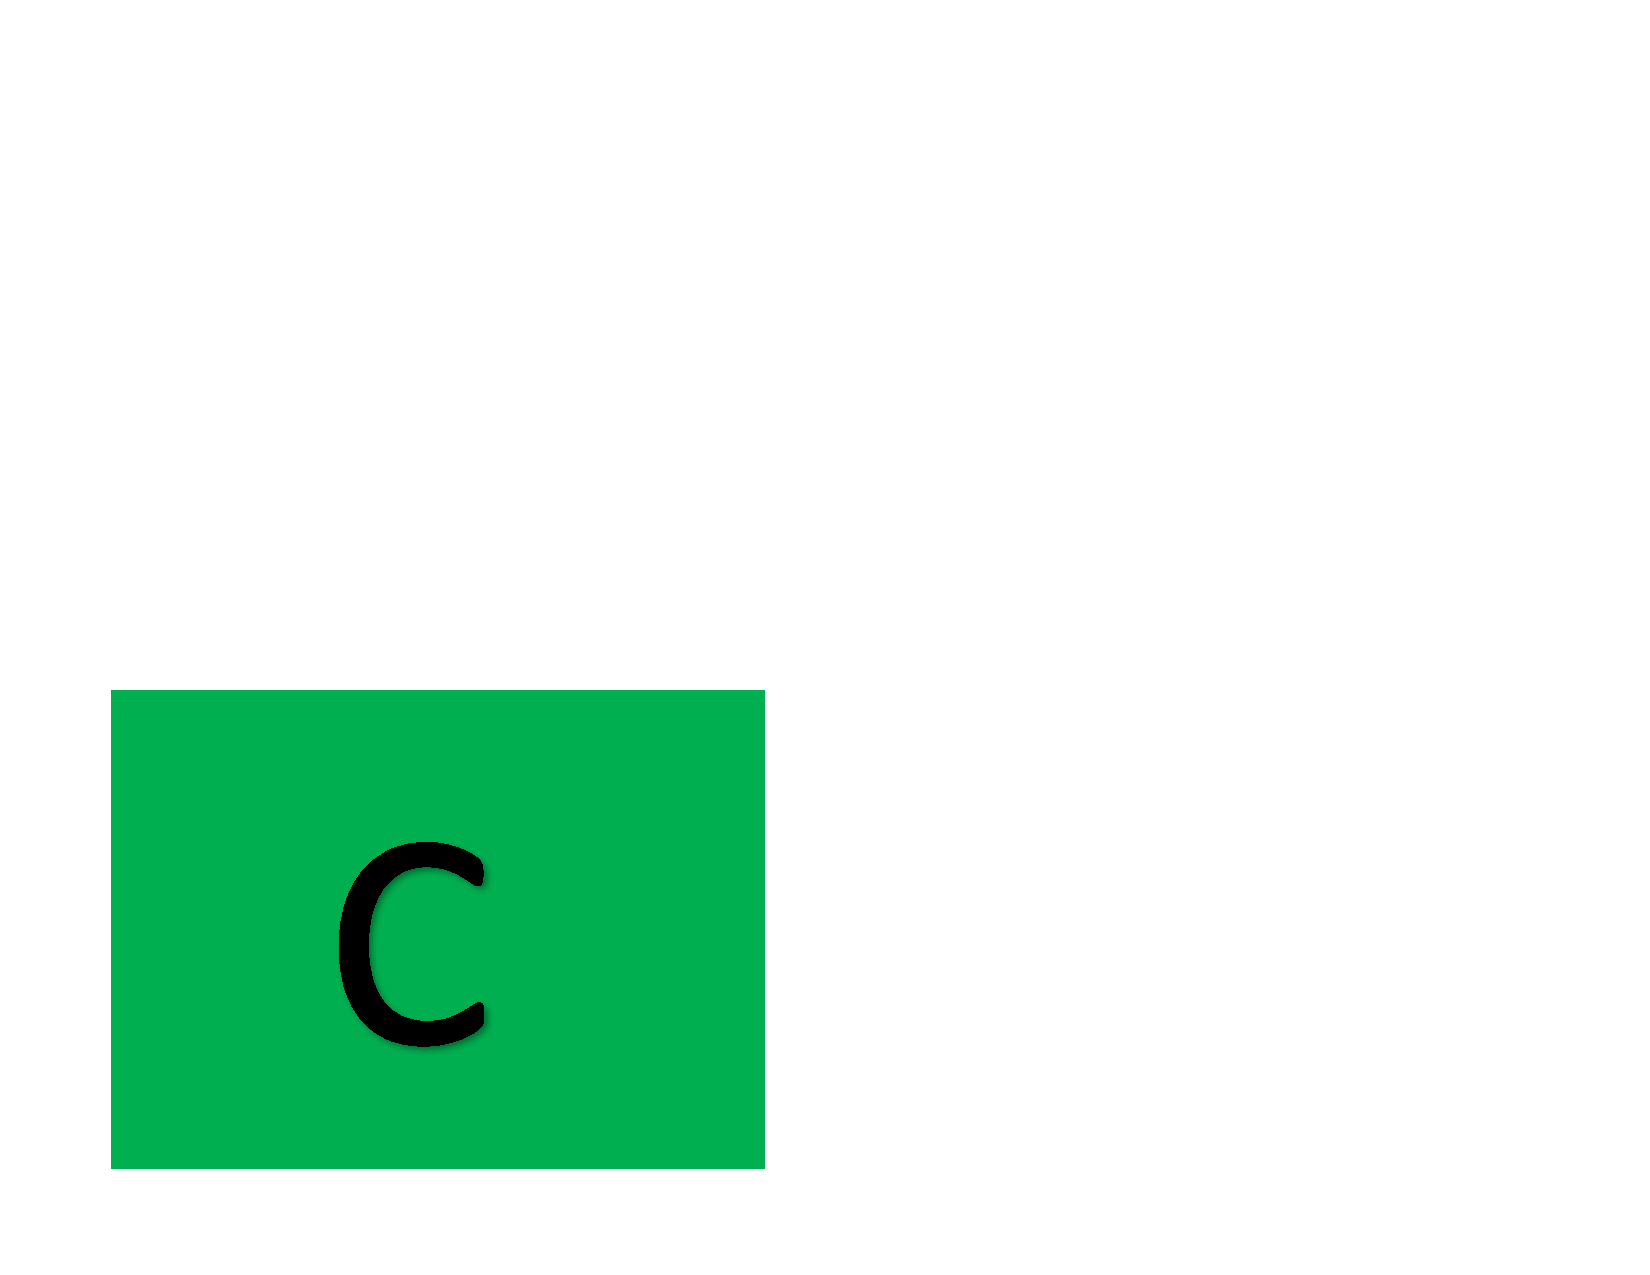
\includegraphics[width=0.8cm,height=0.5cm]{../../Lectures/figures/C}} ]  }
\newcommand*{\ditem}{ \item[{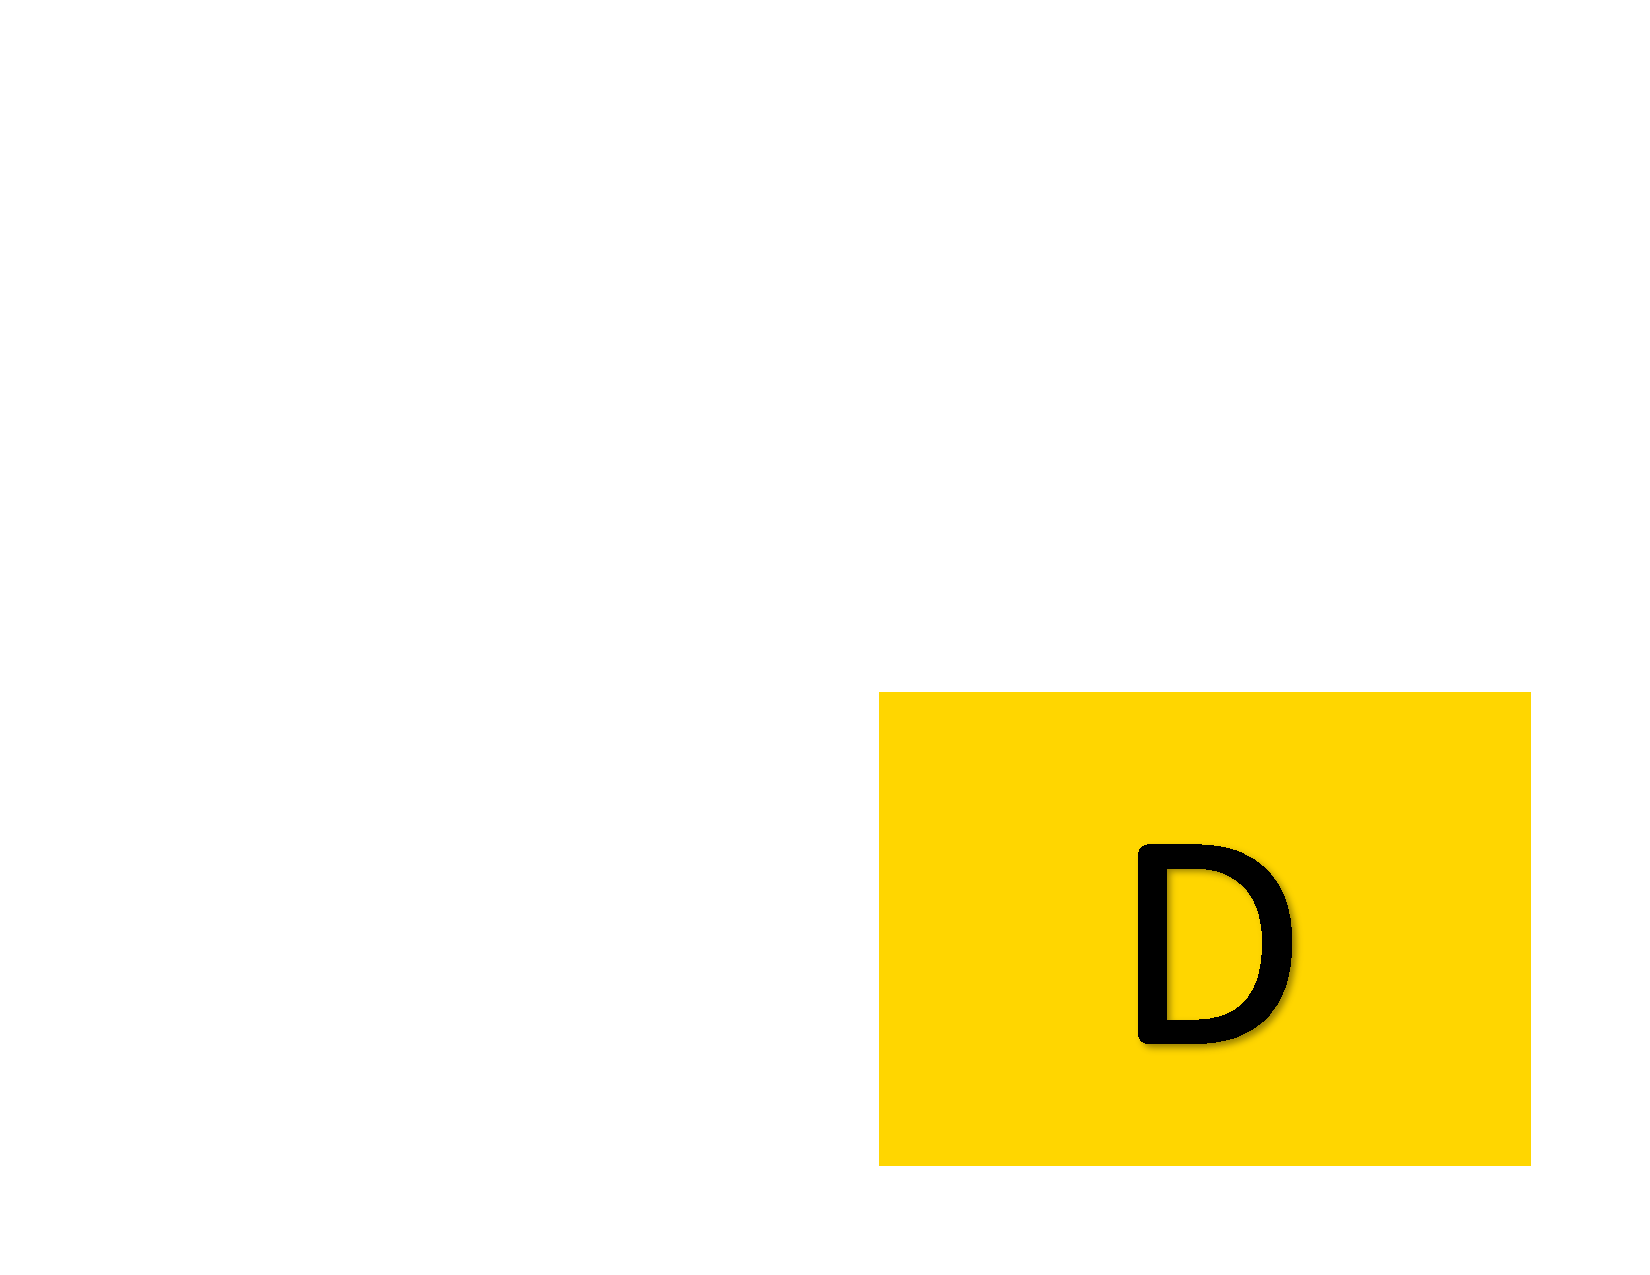
\includegraphics[width=0.8cm,height=0.5cm]{../../Lectures/figures/D}} ]  }
\newcommand*{\eitem}{ \item[{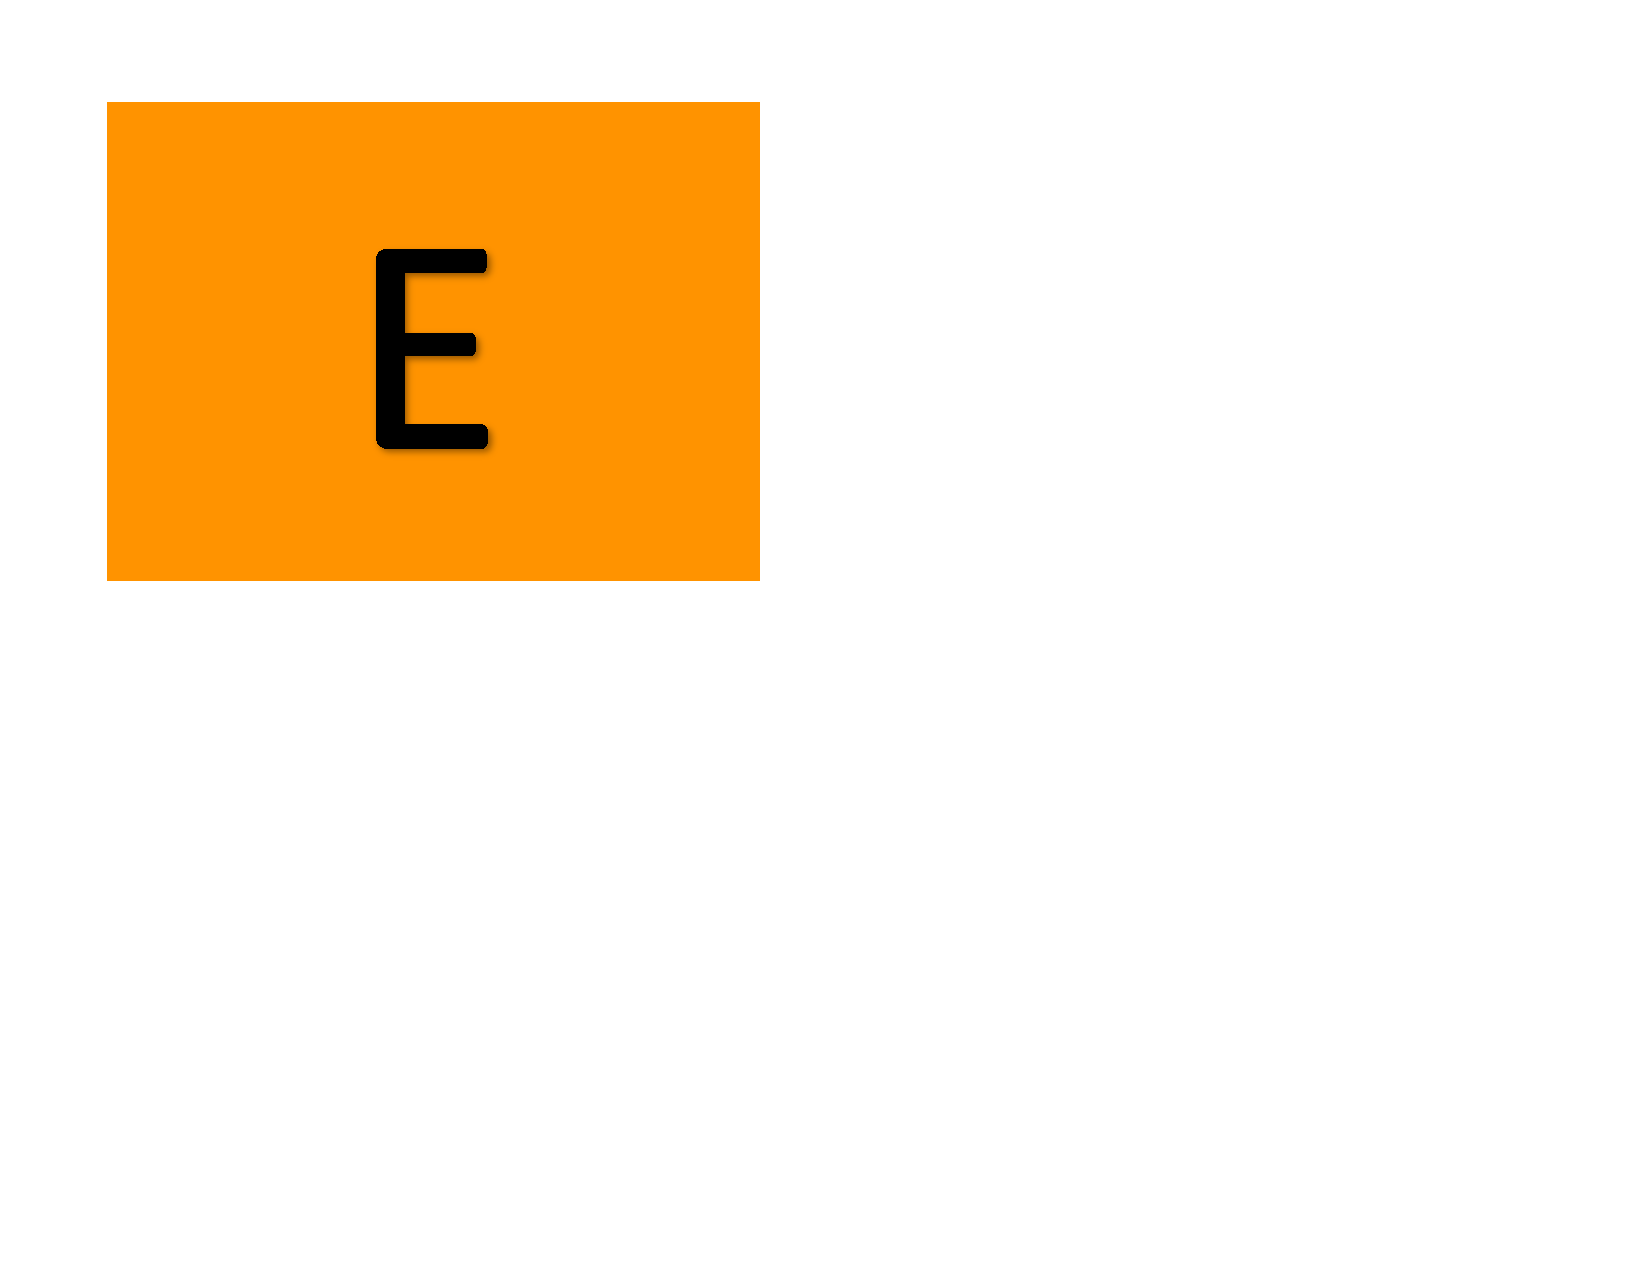
\includegraphics[width=0.8cm,height=0.5cm]{../../Lectures/figures/E}} ]  }
\newcommand*{\fitem}{ \item[{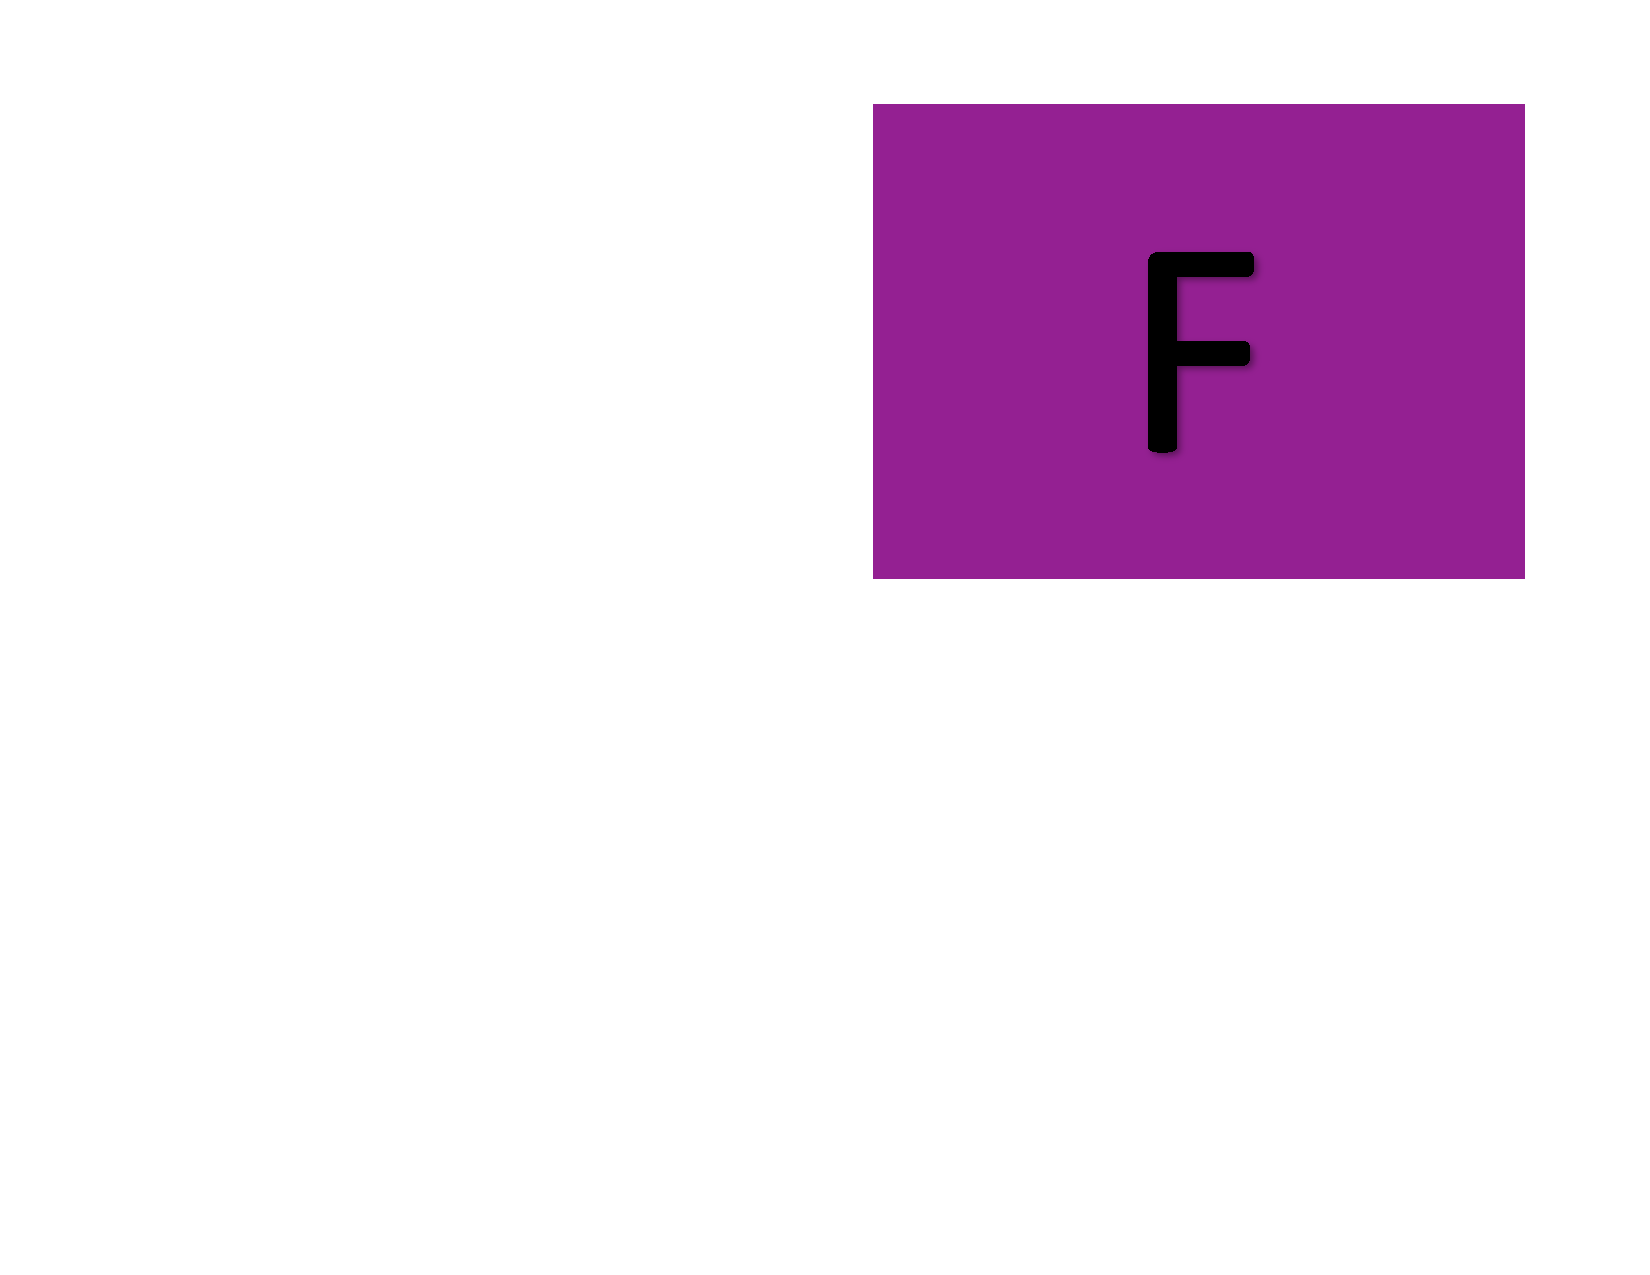
\includegraphics[width=0.8cm,height=0.5cm]{../../Lectures/figures/F}} ]  }


\newcommand{\hide}[1]{\underline{\phantom{#1 #1}}}

\usepackage{setspace}

\onehalfspacing
\newcommand{\tta}{\tt{a}}
\newcommand{\ttb}{\tt{b}}
\newcommand{\ttc}{\tt{c}}
\newcommand{\tte}{\tt{e}}
\newcommand{\ttd}{\tt{d}}
\newcommand{\ttf}{\tt{f}}
\begin{document}
	
	
	\lecture{5: Greedy Algorithms}{January 30, 2025}
	
	\paragraph{Course Logistics}
	
	\begin{itemize}
		\item Greedy algorithms: Chapter 16
		\item Homework 2 is due this Friday (tomorrow)
	\end{itemize}
	

	\section{Making Change}
	Say a cashier has to give someone 68 cents in change to a customer for a purchase. What is the smallest number of coins the cashier can use to give this change, assuming they can give quarters (25 cents), dimes (10 cents), nickels (5 cents) and pennies (1 cent)?\\
	
	\textit{Strategy for giving change:} 
	\begin{itemize}
		\item Choose coins one at a time
		\item At each step, choose the coin \hide{that gets closest} % that gets closest to the total without going over.
	\end{itemize}


	
	\newpage
	\subsection{The Change-Making Problem}
	
	Assume we have $n$ coins, and let
	\begin{align*}
		v_i &=  \hide{ \text{value of the $i$th coin type}} \\ \\
		m_i  &= \hide{\text{number of coins of type $i$}}
	\end{align*}
	
	\paragraph{The Change-Making Problem} Given an integer value $C > 0$ and coin values $$v_1 > v_2 > v_3 > \cdots > v_n = 1,$$ find the number of coins $m_i$ for $i = 1, 2, \hdots n$ so that 
	\begin{itemize}
		\itemsep = 4em
		\item  %$\sum_{i = 1}^n m_i \cdot v_i = C $ \\
		\item %$\sum_{i = 1}^n m_i$ is minimized.
	\end{itemize}
	
	\vs{2cm}
	
	\subsection{The greedy algorithm for change-making} 
	
	
	\begin{algorithm}[b]
		\textsc{GreedyCoinChange}($C$, $v = [v_1, v_2, \hdots , v_n = 1]$)
		\begin{algorithmic}
			\State $n = \text{length}(v)$
			\State Let $m = [0..0]$ be an empty array of $n$ zeros
			\For{$i = 1$ to $n$}
			\While{$C \geq v_i$}
			\State
			\State $m[i] = \hide{m[i] + 1}$
			\State
			\State $C = \hide{C - v_i}$
			\EndWhile
			\EndFor
			\State Return $m$
		\end{algorithmic}
	\end{algorithm}
	
	\newpage
	
	\paragraph{Correctness: The greedy algorithm correctly gives change}
	\begin{proof}
		At each step, we keep updated the amount left that we have to pay. We only add another coin of type $i$ if $v_i$ is less than this amount, so we never go over. We will always reach the exact amount, because $C$ is an integer value and we can always add coins of values $v_n = 1$. 
	\end{proof}
	
	\paragraph{Is the greedy algorithm optimal?}
	
	\QU Which of the following do you think is true?
	\begin{itemize}
		\aitem The greedy algorithm works for some values of $C$ when we use coin values (1,5,10,25) (like $C = 68$), but is sometimes not optimal when we use these coin values (1,5,10,25)
		\bitem The greedy algorithm is always optimal for giving change for coin values (1,5,10,25), but for other coin types $v = (v_1, v_2, \hdots, v_n)$ it may not be optimal
		\citem The greedy algorithm is always optimal for the coin change problem, regardless of coin values, as long as $v_n = 1$. 
		\ditem Any computational problem can be solved optimally by a greedy algorithm
	\end{itemize}
\end{Qu}


%\subsection{Optimality Proofs for Change-Making}
%
%\paragraph{Problem:} For a given coin system $(v_1, v_2, \hdots, v_n = 1)$, determine whether the greedy algorithm for change-making is always optimal. \\
%
%\textit{It turns out that this is a much more general and much more complicated problem!}
%\url{https://www.sciencedirect.com/science/article/abs/pii/S0167637704000823}
%
%This is beyond the scope of our course. Even proving that the greedy strategy is optimal for our (1,5,10,25) coin system is rather tedious, we will not cover it.
%\begin{theorem}
%	The greedy algorithm is optimal for the change-making problem with coin values \hide{$v = (1,5,10,25)$.}
%\end{theorem}

\newpage

\section{Greedy Algorithm Basics}
A greedy algorithm is an algorithm that
\begin{itemize}
	\itemsep = 4em
	\item %Goes through a sequence of steps
	
	\item % Makes a locally optimal solution at each step, i.e., the choice that ``looks best'' at the moment.
\end{itemize}

\vs{1cm} 

\paragraph{Elements of greedy algorithms.} There are two key elements we look for when applying a greedy algorithm:
\begin{enumerate}
	\item \textbf{Optimal substructure}: %same as dynamic programming
	\item \textbf{Greedy-choice property}: a globally optimal solution can be achieved by
	 
	  \hide{making a locally optimal choice.}
\end{enumerate}

\paragraph{Overall strategy for using greedy algorithms}
\begin{enumerate}
	\item Determine a notion of the \hide{``best'' local decision} that improves the global optimization problem.
	\item Show how making one local choice leads to \hide{a smaller subproblem}
	\item Prove that the greedy choice is \hide{``safe''}: it leaves us with a subproblem which, when solves optimally and combined with the first greedy choice, 
	
	\hide{is globally optimal.}
\end{enumerate}

\newpage
%\begin{proof}
%	We can check that for $C< 5$, greedy is always optimal.
%	
%	\vs{2cm}
%	
%	
%	The greedy solution will have a maximum number of 5's possible, followed by the optimal change for 
%	\begin{itemize}
%		\item We know $m_3 \leq 1$, or else replace 1+1 with 2
%		\item We know $m_2 \leq 2$, because 2+2+2 could be replaced by 5+1
%		\item We know $2m_2 + m_3 < 5$, otherwise we could replace 2+2+1 with 5
%		\item 
%	\end{itemize}
%	For $C > 5i$ for an integer $i$, the optimal solution has $m_1 \geq k$, or else we'd violate the previous properties. If we have fewer than $i$ coins of value $v_3 = 5$, then these total to $T \geq 5(i-1)$ and we know we still have to ``pay'' $C - T > 5i - 5(i-1) = 5$. So we have to pay at least a cost of 5 more, but only using coins of value 1 and 2, which cannot be optimal.
%
%\end{proof}

\section{The Activity-Selection Problem}

\paragraph{The activity-selection problem}
Let $(a_1, a_2, a_3, \hdots a_n)$ represent a set of activities, where:
\begin{itemize}
	\itemsep = 3em
	\item $s_i$ = %start time of activity $i$
	\item $f_i$ = % finish time of activity $i$
\end{itemize} 
where $s_i < f_i$ for $i = 1,2,\cdots n$. We assume a half-open interval $[s_i, f_i)$ for the activity $a_i$. Assume these activities are ordered by finish times to that so that

\begin{center}
\hide{$f_1 < f_2 < \hdots < f_n$. }
\end{center}

The activity-selection problem %is to find the largest set of non-overlapping activities. 

\paragraph{Example:}

{\Large
	\begin{tabular}{c | c | c | c | c |  c |}
		$i$ & 1 & 2 & 3 & 4 & 5 \\
		\hline
		$s_i$ & 1 & 3 & 2 & 4 & 7 \\
		\hline
		$f_i$ & 4 & 5 & 6&  8& 9
	\end{tabular} \\
}
\newpage




\subsection{Optimal Substructure}
Consider an activity-selection problem defined by $(a_1, a_2, \hdots , a_n)$ and the time interval $[s_1, f_n)$. If we know that an optimal solution contains activity $a_k$. Then:\\

%An optimal solution can be found by taking $a_k$, and combining it with the  optimal solution on sub-interval $[s_1, f_{k-1})$ and the optimal solution on the sub-interval $[s_{k+1}, f_n)$.

\vs{8cm}


\textbf{A dynamic programming approach:}
Try each $a_k$, solving two smaller subproblems in each case, and taking the best answer. \\

%But what if \emph{we knew a good $a_k$ to choose without trying all of them?}

\newpage


\subsection{A greedy choice lemma}
\begin{lemma}
	There exists an optimal solution to the activity-selection problem defined by $(a_1, a_2, \hdots , a_n)$ that contains $a_1$ (the activity with the earliest finish time).
\end{lemma}
\textit{Proof.}

\begin{itemize}
	\item Let $S$ be an optimal solution, and let $a_i$ be its activity with the earliest start and end time. 
	\item $a_1$ has a finish time $f_1 \leq f_i$. \\
	\item This $a_i$ overlaps with $a_1$, otherwise we could add $a_1$ to make $S$ better\\
	\item If we replace $a_i$ with $a_1$ to get $S'$, then $|S| = |S'|$, and this is a valid non-overlapping solution, because $a_i$ was the earliest activity in $S$.
\end{itemize}

\newpage
\subsection{An Optimal Greedy Algorithm for the Activity-Subset Problem}

\begin{algorithm}
	\textsc{GreedyActivitySelection}($s = (s_1, s_2, \hdots , s_n)$, $f = (f_1, f_2, \hdots , f_n)$)
	\begin{algorithmic}
		\State $n = \text{length}(s)$
		\State $S = \{a_1\}$
		\State $k = 1$		\;\;\;  %	//$f_k$ is the finish of the last added activity
		\For{$i = 2$ to $n$}
		\If{$s_i \geq f_k$}		 %// only consider activities that start after the last one ends.
		\State  %//Note: this is not saying we take the first activity that starts after $a_k$!
		\State $S = S \cup \{a_i\}$
		\State 
		\State $k = i$
		\State
		\EndIf
		\EndFor
		\State Return $S$
	\end{algorithmic}
\end{algorithm}

%\paragraph{Example}


\newpage

\section{Binary Codes}

%	In binary code compression, the goal is to compress a string of characters efficiently using 0's and 1's.
\begin{itemize}
	\item An \hide{alphabet  } is a set of characters, e.g., $C = \{\tt{a},\tt{b}, \tt{c},\tt{d} ,\tt{e}, \ttf\}$ \\
	\item A \emph{binary code} for $C$ is\\ %a way to represent each $c \in C$ using a binary string.
\end{itemize}

Consider three possible codes for $C = \{\tt{a},\tt{b}, \tt{c},\tt{d} ,\tt{e}, \ttf\}$.
\begin{equation}
	\label{tab1}
	\begin{tabular}{c c c c c c c}
		Character: &  \tta & \ttb & \ttc & \ttd & \tte & \ttf \\
		\hline
		example code 1: & 000 & 001 & 010 &  011 & 100 & 101 \\
		example code 2: &0 & 101 & 100 & 111 & 1101 & 1100 \\
		example code 3: &0 & 1 & 10 & 01 & 11 & 00 \\
		\hline
	\end{tabular} \\
\end{equation}

Types of codes:
\begin{itemize}
	\item \textbf{Fixed length code}: %all codes have the same length
	\item \textbf{Variable-length code}: %codes can have different lengths (but are still unique)
	\item \textbf{Prefix code}: the codeword for every $c \in C$ is % \emph{not} the start of any other codeword
\end{itemize}

\QU 
Which of the codes in Table~\ref{tab1} is a prefix code?
\begin{itemize}
	\aitem Example code 1
	\bitem Example code 2
	\citem Example code 3
	\ditem Example codes 1 and 2
	\eitem Example codes 1, 2, and 3
\end{itemize}
\end{Qu}

\newpage 

\subsection{Encoding and Decoding}
Consider a string of characters from the alphabet $C = \{\tt{a},\tt{b}, \tt{c},\tt{d} ,\tt{e}, \ttf\}$ where the frequency of each character is given in the following table and we have two codes.
\begin{equation}
\begin{tabular}{c c c c c c c}
	Character: &  \tta & \ttb & \ttc & \ttd & \tte & \ttf \\
	\hline
	Frequency & 0.45 & 0.13 & 0.12 & 0.16 & 0.09 & 0.05 \\
	FLC: & 000 & 001 & 010 &  011 & 100 & 101 \\
	VLC: &0 & 101 & 100 & 111 & 1101 & 1100 \\
	\hline
\end{tabular} 
\end{equation}
\newpage


\subsection{The Optimal Prefix Code Problem}

\paragraph{The optimal prefix code problem} Given an alphabet $C$ and a frequency $\mathit{c.freq}$ for each $c \in C$ in a given string $s$,  \\ \\ %find the prefix code that represents $s$ using a minimum number of bits. \\


\paragraph{Representing a prefix code as a tree}
Every prefix code for a string $s$ can be represented as a binary tree $T$ where 
\begin{itemize}
\item Left branches are associated with %`0'
\item Right branches are associated with %`1'
\item Each leaf corresponds to a character $c \in C$, whose binary code is given by \\
%the bits in the path from the root to the leaf
\item Each node is associated with the frequency of characters in its subtree
\end{itemize}

\paragraph{Example}
\begin{tabular}{c c c c c c c}
Character: &  \tta & \ttb & \ttc & \ttd & \tte & \ttf \\
\hline
Frequency & 0.45 & 0.13 & 0.12 & 0.16 & 0.09 & 0.05 \\
VLC: &0 & 101 & 100 & 111 & 1101 & 1100 \\
\hline
\end{tabular} 

\newpage

The cost of the tree is give by \\
\begin{equation*}
B(T) = \sum_{c \in C} \\%\mathit{c.freq} \cdot d_T(c)
\end{equation*}
where $d_T(c)$ is the depth of $c$ in the tree $T$. 

\QU
True or false: every binary tree (with $\ell$ leaves) gives a valid prefix code (for an alphabet with $\ell$ characters).
\begin{itemize}
\aitem True
\bitem False
\end{itemize}
\end{Qu}


\newpage

\begin{theorem}
%Any binary tree with $|C|$ leaves gives a valid prefix code for $C$.
\end{theorem}
\vs{1.5cm}
\textit{Proof.}

\vfill



\paragraph{Optimal prefix code problem:} 

\vs{1cm}
%Find the binary tree representation %with minimum cost. 


\paragraph{Nice properties about the optimal tree}
In the optimal tree representation,
\begin{itemize}
\itemsep = 3em
\item %There are $|C|$ leaves
\item %Each node in the tree has a sibling
\end{itemize}



\newpage

\subsection{Huffman Codes}
Huffman Code: a prefix code obtained by greedily building a tree representation for $C$

%\textbf{Input:} Alphabet $C$, for each $c \in C$, a frequency $c.freq$.\\
%\textbf{Output:} A binary tree representing a prefix code

\paragraph{Huffman Code Tree Process}
\begin{itemize}
	\item Associate each character in $C$ with a node, labeled by its frequency
	\item Identify two nodes $x$ and $y$ in $C$ with the \hide{smallest frequencies}
	\item Create new node $z$ with frequency \hide{$z.freq = x.freq + y.freq$.}
	\item Make $z.left = x$, and $z.right = y$.
	\item Repeat the above procedure on the alphabet obtained by \hide{replacing $x$ and }\\
\end{itemize}
Observe: $x$ and $y$ will be siblings in $T$ at \hide{a maximum depth.}
\paragraph{Activity} Create a Huffman code for:
\begin{tabular}{c c c c c c c}
	Character: &  \tta & \ttb & \ttc & \ttd & \tte & \ttf \\
	\hline
	Frequency & 0.45 & 0.13 & 0.12 & 0.16 & 0.09 & 0.05 
\end{tabular} 

\newpage

\subsection{Code and Illustration}
\begin{algorithm}[t]
	\textsc{HuffmanCode}($C$)
	\begin{algorithmic}
		\State $n =|C|$
		\State $T \leftarrow$ empty graph 
		\State $Q \leftarrow \emptyset$ 
		\For{$c$ in $C$}
		\State Insert $c$ with value $c.freq$ into $T$ and $Q$
		\EndFor
		\For{$i = 1$ to $n-1$}
		\State $x = $ % \textsc{ExtractMin}(Q)$
		\State $y = $ %\textsc{ExtractMin}(Q)$
		\State create node $z$
		\State 
		\State 
		\State 
		\State
		\State 
		\State
		\State 
		%			\State Insert $z$ into $T$
		%			\State Insert $z$ into $Q$ with frequency $z.val$
		\EndFor
		\State Return $T$
	\end{algorithmic}
\end{algorithm}
\newpage

\subsection{Runtime Analysis}
Given a set of objects $C$, with values $c.val$ for $c \in C$ and $n = |C|$, a binary min-heap for $C$ is a binary tree such that
\begin{itemize}
	\item All levels %(except maybe the last) are complete
	\item The value of a node is % $\leq$ the value of its descendants.
\end{itemize}
It has the following operations:
\begin{itemize}
	\item $\textsc{BuildBinMinHeap}(C)$:  \\% builds heap $Q$ from elements in $C$, takes $O(n)$ time.
	\item $\textsc{ExtractMin}(Q)$: \\
	
	%removes minimum element. Takes $O(\log n)$ time.
	\item $\textsc{Insert}(Q,z,z.freq)$: \\ %adds an element to $Q$. Takes $O(\log n)$ time.
\end{itemize}

\QU
Assume we use a binary min heap to store and update $Q$ in the pseudocode above. Then what is the overall runtime of creating a Huffman code, in terms of $n = |C|$?
\begin{itemize}
	\aitem $O(\log n)$
	\bitem $O(n)$
	\citem $O(n \log n)$
	\ditem $O(n^2)$
\end{itemize}
\end{Qu}


\pagebreak

\subsection{Optimality}
It turns out that a Huffman code optimally solves the prefix code problem. The argument hinges on the following lemma.

\begin{lemma}
Let $C$ be an alphabet where $c.freq$ is the frequency of $c \in C$. Let $x$ and $y$ be the two characters in $C$ that have the lowest frequencies. \\

Then, there exists an optimal prefix code for $C$ in which $x$ and $y$ have the same length code words and only differ in the last bit. \\

Equivalently: \\% there exists a Huffman code tree in which $x$ and $y$ are sibling leaves at maximum depth.
\end{lemma}



\newpage 
\paragraph{Why does this imply optimality?}
Consider a slightly different (but equivalent) approach to defining a Huffman code:
\begin{enumerate}
\item Associate each character with a node, labeled by its frequency
\item Identify the two nodes $x$ and $y$ with the smallest frequencies
\item Create new node $z$ with frequency $z.freq = x.freq + y.freq$. 
\item  %Let $T'$ be an optimal tree for alphabet $C'$ obtained by replacing $x$ and $y$ with $z$
\item Create tree $T$ from $T'$ by making $z.left = x$, and $z.right = y$.
\end{enumerate}

\paragraph{Claim}
This produces an optimal tree $T$. 

\textit{Proof.}
Note that the cost of the tree $T$ is 
\begin{equation}
\label{this}
B(T) = B(T') + x.freq + y.freq
\end{equation}

\vs{2cm}

%	Why? Because instead of a node $z$ of depth $d$, we have nodes $x$ and $y$ at depth $d+1$, so for two characters, the codeword is 1 longer. \\ 

We prove the result by contradiction: suppose that $T$ is not optimal. Then %there exists some tree $R$ that is better,

%$$B(R) < B(T)$$

\vs{2cm}

We can assume that $x$ and $y$ are at maximum depth in $R$. \\

%	
Let $R'$ be the tree obtained by taking $R$ and \\ %replacing $x$ and $y$ with a merged node $z$. 

Similar to~\eqref{this} we have that:  \\


We then get an impossible sequence of inequalities:
\begin{align*}
B(R') &= B(R) - x.freq - y.freq \\
& < B(T) - x.freq - y.freq \\
& = B(T') 
\end{align*}

%	This says that $R'$ is a strictly better tree for $C'$, but we said $T'$ was optimal for $C'$. Contradiction!


\end{document}
